%Auteurs : Enes Ulusoy
\documentclass[british,french,11pt, a4paper, openany]{book}

% Règles de bonne pratiques :
% https://fr.wikibooks.org/wiki/LaTeX/Gestion_des_gros_documents

%%%%%%%%%%%%%%%%
%%% Packages %%%
%%%%%%%%%%%%%%%%

%%% Général %%%
\usepackage[utf8]{inputenc}   
\usepackage[french]{babel}
\usepackage[T1]{fontenc}
\usepackage{mathpazo}
\usepackage{lmodern}
\usepackage{courier}
\usepackage{graphicx}
\usepackage{cancel}

%%% Tableau %%%
\usepackage{tabularx} %Permet d'auto dimensionner les tableaux



%%% Bibliographie %%%
\usepackage[style=alphabetic,backend=bibtex]{biblatex}
\usepackage[autostyle]{csquotes}
\DeclareNameAlias{sortname}{last-first}
\DeclareFieldFormat{url}{\space\url{#1}}
\DeclareNameAlias{labelname}{last-first}
\addbibresource{sample.bib}


%%% Graphiques %%%
\usepackage{tikz}
\usepackage{pgfplots}
\usepackage{circuitikz}

%%% Mise en page %%%
\usepackage{amsmath}
\usepackage{amsfonts}
\usepackage{amssymb}
\usepackage{amsthm}
\usepackage[tt]{titlepic}% Centre le titre
\usepackage{fancyhdr}   % Permet de modifier l'entête & footer
\usepackage{caption}     % Permet d'ajouter des légendes en images sans les mettre en float + dans la marge + ref vers le haut de l'envirronement
\usepackage{wrapfig}
\usepackage{fullpage}
\usepackage{multicol}   % pour les liste sur plusieurs colonnes
\usepackage{subfigure}  % alligne deux images cote a cote
\usepackage{float}      %permet de mettre du texte entre les figures grace a [H]. Génial! 
\usepackage{eso-pic}    % Fond d'écran page de garde
\usepackage{adjustbox}  % Empêche les box de sortir de la page


%%% Math %%%
\usepackage{delarray} % Belles matrices
\usepackage{siunitx}
\sisetup{locale = FR,detect-all}
% Pour mettre siunitx en mode français (virgule plutôt que point etc.)

%%% Codes %%%
\usepackage{listings}
\usepackage[final]{pdfpages} %% Inclusion fichier pdf

%% Reference
\usepackage{hyperref}
\renewcommand*{\figureautorefname}{fig.}
\def\appendixautorefname{annexe}
\def\tableautorefname{tab.}
\renewcommand*{\chapterautorefname}{ch.}




%%%%%%%%%%%%%%%%%
%%% Commandes %%%
%%%%%%%%%%%%%%%%%

%%% Physique %%%
\newcommand{\cst}{\text{cst}}
\newcommand{\D}{\partial}
\newcommand{\E}{\vec E}
\newcommand{\B}{\vec B}
\newcommand{\F}{\vec F}
\newcommand{\modu}[1]{|$#1$|}

%%% Math %%%
\newcommand{\oiint}{\int\!\!\!\!\!\!\! \:\!\subset\!\!\supset\!\!\!\!\!\!\!\int}
\newcommand{\rot}{\text{rot}\,}
\newcommand{\divv}{\text{div}\,}
\newcommand{\phas}[1]{\underline{#1}}
\newcommand{\RE}{\text{Re}}
\newcommand{\ft}{\overset{\mathcal{F}}{\longleftrightarrow}}
\newcommand{\lt}{\overset{\mathcal{L}}{\longleftrightarrow}}




%% Box
\newcommand{\theor}[1]{\adjustbox{minipage=\linewidth-2\fboxsep-2\fboxrule,fbox}{\textsc{Théorème : }#1}}
\newcommand{\defi}[1]{\adjustbox{minipage=\linewidth-2\fboxsep-2\fboxrule,fbox}{\textsc{Définition : }#1}}
\newcommand{\lemme}[1]{\adjustbox{minipage=\linewidth-2\fboxsep-2\fboxrule,fbox}{\textsc{Lemme : }#1}}
\newcommand{\prop}[1]{\adjustbox{minipage=\linewidth-2\fboxsep-2\fboxrule,fbox}{\textsc{Propriété}\\ #1}}
\newcommand{\proposition}[1]{\adjustbox{minipage=\linewidth-2\fboxsep-2\fboxrule,fbox}{\textsc{Proposition}\\#1}}
\newcommand{\retenir}[1]{\adjustbox{minipage=\linewidth-2\fboxsep-2\fboxrule,fbox}{\textbf{\textit{\textsc{A retenir} : }}#1}}
\newcommand{\corollaire}[1]{\ \\\begin{tabular}{||c}
	\begin{minipage}{\textwidth}
		\textsc{Corollaire : } \textit{#1}
	\end{minipage}
	\end{tabular}}
\newcommand{\exemple}[1]{\ \\\begin{tabular}{|c}
	\begin{minipage}{\textwidth}
		\textsc{Exemple : } #1
	\end{minipage}
	\end{tabular}}
    
    

%\pagestyle{headings} % Titre du ch et numéro page dans l'entete
\renewcommand{\proofname}{Démonstration}
\selectlanguage{french}

\addto\captionsfrench{\def\tablename{Tableau}}


%%% Background %%%
\newcommand\BackgroundPic{%
	\put(0,0){%
		\parbox[b][\paperheight]{\paperwidth}{%
			\vfill
			\centering
			
\includegraphics[width=\paperwidth,height=\paperheight,%
			keepaspectratio]{../../Builder/ulb.jpg}%
			\vfill
}}}

%%% Annexes Cedu %%%
%\usepackage{calrsfs}
\DeclareMathAlphabet{\pazocal}{OMS}{zplm}{m}{n}
\usepackage{fourier-orns}

\setlength{\parindent}{0pt} 

%%% Attributs %%%
\newcommand*{\NomduCours}[2]{\def\cours{#1}\def\memo{#2}}
\newcommand*{\auteur}[2]{\def\prenom{#1}\def\nom{#2}}
\newcommand*{\rappeltheo}[2]{\def\rappeltheoprenom{#1}\def\rappeltheonom{#2}}
\newcommand*{\professeur}[2]{\def\pprenom{#1}\def\pnom{#2}}
\newcommand*{\sprofesseur}[2]{\def\spprenom{#1}\def\spnom{#2}}
\newcommand*{\annee}[2]{\def\adebut{#1}\def\afin{#2}}
% Attributs
\NomduCours{Structural Analysis \& Finite Elements}{MECA-H421}
\addauteur{Enes}{Ulusoy}
\addprofesseur{Pyl}{Lincy}
\addprofesseur{Peter}{Berke}
\annee{2016}{2017}
\renewcommand{\theor}[1]{\adjustbox{minipage=\linewidth-2\fboxsep-2\fboxrule,fbox}{\textsc{}#1}}
\newcommand{\uinf}{u_\infty}
\usepackage{mathtools}
\usepackage{multicol}
\usepackage{bm}

% Document
\begin{document}
\selectlanguage{british}
\def\equationautorefname~#1\null{%
		(#1)\null
	}
%%%%%%%%%%%%%%%%%
% Préliminaires %
%%%%%%%%%%%%%%%%%
\frontmatter
\AddToShipoutPicture*{\BackgroundPic}

\begin{titlepage}
	\begin{center}	
			
		\newcommand{\HRule}{\rule{\linewidth}{0.5mm}}   			            %Titre en gros
		
\includegraphics[scale=0.11]{../../Builder/titlepage/logo.jpg}~\\[1cm]				%Logo
			
			\textsc{\LARGE Université Libre de Bruxelles}\\[1.5cm]
			\textsc{\Large Synthèse}\\[0.5cm]
			
			\HRule \\[0.4cm]
			{ \huge \bfseries \cours \ \\\memo \\[0.4cm] }
			
			
			\HRule \\[1.5cm]
			\begin{minipage}[t]{0.6\textwidth}
				\begin{flushleft}%\large
					\emph{Auteur :}\\
					\mbox{\prenom~\textsc{\nom}}\\
					\ifdefined\nnom
					\ \\
					\emph{Notes :}\\
					\mbox{\nprenom~\textsc{\nnom}}\\
					\fi
					\ifdefined\rappeltheonom
					\ \\
					\emph{Rappels théoriques :}\\
					\mbox{\rappeltheoprenom~\textsc{\rappeltheonom}}
					\fi 
				\end{flushleft}
			\end{minipage}
			\begin{minipage}[t]{0.25\textwidth}
				%\begin{flushright}
				%\large
				\emph{Professeur :}\\
				\mbox{\pprenom~\textsc{\pnom}}
				\ifdefined\spprenom
				\\ \mbox{\spprenom~\textsc{\spnom}} \\
				\fi
				%\end{flushright}
			\end{minipage}
			
			\vfill
			
			% Bottom of the page
			{\large Année \adebut~-~\afin}
			
		\end{center}
	\end{titlepage}

\chapter*{Appel à contribution}
\subsection*{Synthèse Open Source}
\begin{wrapfigure}[5]{l}{4.5cm}
	
\includegraphics[scale=0.5]{../../Builder/git.png}
\end{wrapfigure}
Ce document est grandement inspiré de l’excellent cours donné 
par \pprenom~\pnom\	
\ifdefined\spprenom
et\ \spprenom~\spnom\ 
\fi
 à l’EPB (École Polytechnique de Bruxelles), faculté de l’ULB (Université 
Libre de Bruxelles). Il est écrit par les auteurs susnommés avec l’aide de tous les autres étudiants 
et votre aide est la bienvenue ! En effet, il y a toujours moyen de l’améliorer surtout que si le 
cours change, la synthèse doit être changée en conséquence. On peut retrouver le code source à l’adresse 
suivante
\begin{center}
	\url{https://github.com/nenglebert/Syntheses}
\end{center}\ \\
Pour contribuer à cette synthèse, il vous suffira de créer un compte sur \textit{Github.com}. De
légères modifications (petites coquilles, orthographe, ...) peuvent directement être faites sur le
site ! Vous avez vu une petite faute ? Si oui, la corriger de cette façon ne prendra que quelques 
secondes, une bonne raison de le faire ! \\
\\
Pour de plus longues modifications, il est intéressant de disposer des fichiers : il vous 
faudra pour cela installer \LaTeX, mais aussi \textit{git}. Si cela pose problème, nous sommes 
évidemment ouverts à des contributeurs envoyant leur changement par mail ou n’importe quel autre 
moyen.\\
\\
Le lien donné ci-dessus contient aussi le \texttt{README} contient de plus amples informations, 
vous êtes invités à le lire si vous voulez faire avancer ce projet ! 

\subsection*{Licence Creative Commons}
\begin{wrapfigure}[3]{r}{2.8cm}
	\vspace{-5mm}
	
\includegraphics[scale=0.17]{../../Builder/CC}
\end{wrapfigure}
Le contenu de ce document est sous la licence Creative Commons : \textit{Attribution-NonCommercial-ShareAlike 
4.0 International (CC BY-NC-SA 4.0)}. Celle-ci vous autorise à l'exploiter pleinement, compte-
tenu de trois choses :
\begin{enumerate}
	\item \textit{Attribution} ; si vous utilisez/modifiez ce document vous devez signaler le(s) nom(s)
	      de(s) auteur(s).
	\item \textit{Non Commercial} ; interdiction de tirer un profit commercial de l’œuvre sans 
	      autorisation de l'auteur 
	\item \textit{Share alike} ;  partage de l’œuvre, avec obligation de rediffuser selon la même 
	      licence ou une licence similaire
\end{enumerate}
Si vous voulez en savoir plus sur cette licence :
\begin{center}
	\url{http://creativecommons.org/licenses/by-nc-sa/4.0/}
\end{center}

\begin{flushright}
	\textbf{Merci ! }
\end{flushright}
\tableofcontents
%Si abstract, \input ici

%%%%%%%%%%%%%%%%%%%%%
% Contenu principal %
%%%%%%%%%%%%%%%%%%%%%
\mainmatter

\setcounter{chapter}{1}
%%%%%%%%%%%%%%%%%%%%%%%%%%%%%%%%%%%%%
% Ch2 : Les liaisons interatomiques %
%%%%%%%%%%%%%%%%%%%%%%%%%%%%%%%%%%%%%

\chapter{Liaisons interatomiques}
\section{La liaison}
Le but des liaisons est de remplir la couche de valence et de se rapprocher au plus de la configuration des gaz rares. L'existence de composés polyatomiques stables implique que les atomes soient capable de former des agrégats dont \textbf{l'énergie est plus faible que s'ils étaient isolés}. Les types de liaison dépendent de l'agencement des électrons de valence et sont au nombre de 4 : \\

\begin{itemize}
	\item[•] la liaison ionique
	\item[•] la liaison covalente
	\item[•] la liaison métallique
	\item[•] les liaisons secondaires hydrogène et de Vander Waals. \\
\end{itemize}
	
Les 3 premières sont des liaisons fortes alors que les dernières sont plus faibles. Soulignons que, le plus souvent, la liaison des atomes dans un solide présente un caractère mixte associant des contributions simultanées de plusieurs types liaisons chimiques.
	
\section{La liaison ionique, opportunisme individualiste}
Type de liaison qui détermine la cohésion des solides constitués de l'association d'atomes possédant des affinités électronique très différentes. Prenons l'exemple du sel de cuisine $NaCl$ et regardons ce qui se passe d'un point de vue énergétique. Tout d'abord, l'énergie de première ionisation de $Na$ et l'affinité électronique (énergie libéré lorsqu'un électron est capté) de $Cl$ sont
\begin{equation}
	E_{ion}\, Na= 5.14 \, eV \qquad et \qquad \mbox{Aff.élec } Cl = 4.02 \, eV 
\end{equation}	 
ce qui veut dire qu'il faut $U_i = 1.12\, eV$ pour séparer $NaCl$ en $Na^++Cl^-$. Il faut encore tenir compte de la force électrostatique $F$ entre les deux ions de charges différentes. Quand un ion se rapproche depuis l'infini, 
\begin{equation}
	U_a = \int _\infty ^r F_{attr} \, dr= \int _\infty ^r \frac{q^2}{4\pi \epsilon _0 r^2} \, dr = -\frac{q^2}{4\pi \epsilon _0 r}
\end{equation}
Le signe négatif de cette énergie traduit le fait que les ions ont tendance à se rapprocher. Cependant, à très petite distance, les cortèges électroniques commencent à se superposer et une forte répulsion apparaît selon 
\begin{equation}
	U_r = \frac{B}{r^n}
\end{equation}
\begin{wrapfigure}[5]{l}{6.5cm}
	\vspace{-5mm}
	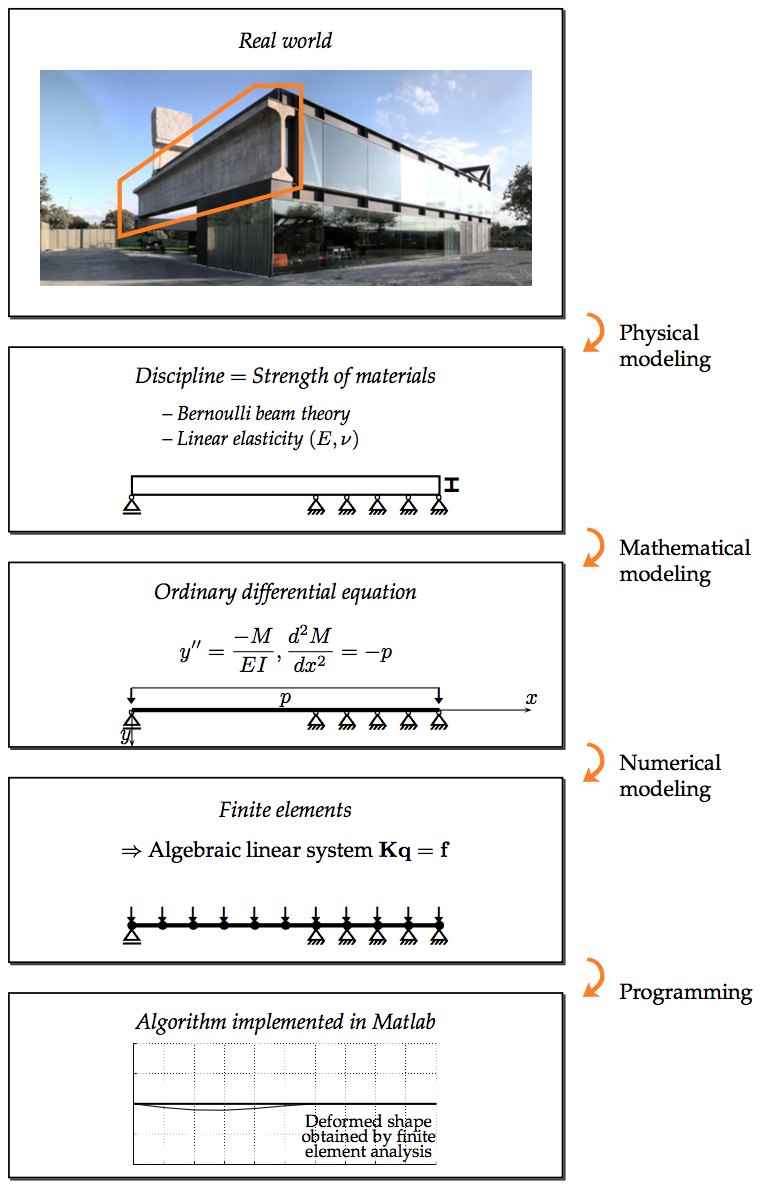
\includegraphics[scale=0.6]{ch2/1}
\end{wrapfigure}
La somme de toutes ces contributions donne la courbe d'énergie potentielle suivante. 
A SUIVRE
\chapter{Traction - Compression}
\section{Traction}
	\subsection{Méthode cinématique}
	\begin{wrapfigure}[8]{r}{6.5cm}
	\vspace{-5mm}
	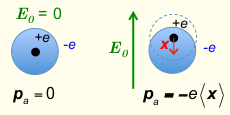
\includegraphics[scale=0.4]{ch3/image1.png}
	\captionof{figure}{ }
	\end{wrapfigure}
	Nous allons ici utiliser la méthode cinématique de sorte que les équations 
	de compatibilité soient satisfaites lors de l'obtention de notre relation 
	contrainte $\leftrightarrow N$. Il faut donc postuler un champ de 
	déplacement :
	\begin{equation}
	u = u_0(x),\qquad v=0,\qquad w=0.
	\end{equation}
	On considère un déplacement axial $u$, uniquement selon $x$ : ne varie 
	pas selon $x$ et $y$ et constante dans toute la section : une section 
	transversale plane, reste plane\footnote{hypothèse de Bernoulli (1694) :
	les sections droites initialement planes et perpendiculaires à l'axe le 
	restent dans la configuration déformée}.
	
	\subsection{Déplacements - Déformations - Contraintes}
		\subsubsection{Déformations}
		Maintenant que nous avons notre déplacement, il faut s'intéresser 
		aux déformations :
		\begin{equation}
		a_{ij} = \frac{1}{2}\left(\dfrac{\partial u_i}{\partial x_j}+\dfrac{
		\partial u_j}{\partial x_i}\right)
		\end{equation}
		De par notre champ, $\epsilon_x$ est constant dans la section 
		transversale et les autres composantes sont nulles :
		\begin{equation}
		\epsilon_x = \dfrac{\partial u_0}{\partial x}
		\end{equation}
		
		\subsubsection{Contraintes}
		On utilise pour ça la loi de Hooke $ \sigma_x = E\epsilon_x$. Notons 
		que si $E$ est constant, $\sigma_x$ l'est dans la section transversale.
		On néglige les composantes de Poisson.
		
	\subsection{Éléments de réduction : section homogène}
	La suite de notre méthode demande le calcul des éléments de réductions. 
	Supposons que l'on ai une section homogène de sorte que $E$ soit constant. 
	Dès lors, $\sigma_x$ est également constant. Pour la normale, c'est immédiat :
	\begin{equation}
	N = \int_A \sigma_x\ dA \qquad\Longrightarrow\qquad N = \sigma_xA
	\end{equation}
	En raison de notre champ uniquement selon $x$, les résultantes en $y$ et $z$ 
	sont nulles, de même pour le moment selon $x$\\
		\begin{wrapfigure}[7]{l}{6.5cm}
	\vspace{-5mm}
	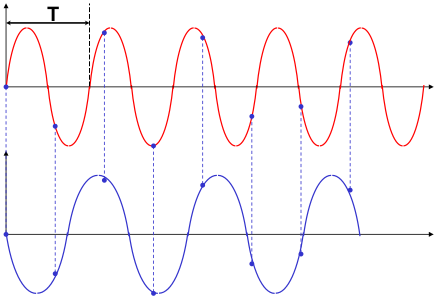
\includegraphics[scale=0.45]{ch3/image2.png}
	\captionof{figure}{ }
	\end{wrapfigure}
	\begin{equation}
	\begin{array}{ll}
	R_y = \int_A \tau_{xy}\ dA &\Longrightarrow T_y = 0\\
	\text{Similairement : }&\Longrightarrow T_z = 0\\
	C_x = \int_A (\tau_{xz}y-\tau_{xy}z)\ dA &\Longrightarrow M_x = 0
	\end{array}
	\end{equation}
	Pour le moment selon $y$ (et similairement pour $z$) nous avons :
	\begin{equation}
	C_y = \int_A \sigma_xz\ dA\qquad\Longrightarrow\qquad C_y =  \sigma_x
	\int_A z\ dA
	\end{equation}
	Si l'origine des axes est le \textbf{centre géométrique}\footnote{Centre 
	de "gravité" sans masse.} défini tel que 
	\begin{equation}
	\int_A y\ dA = 0,\qquad \int_A z\ dA = 0.
	\end{equation}
	ALors, $M_y$ et $M_z$ sont nuls.
	
		\subsubsection{En résumé}
		La poutre est uniquement soumise à un effort \textbf{normal} (et pas 
		un fléchissant). Pour une poutre de section homogène ($E$ constant), 
		nous avons une distribution uniforme de la contrainte axiale 
		\begin{equation}
		\sigma_x = \dfrac{aN}{A}
		\end{equation}
		Pour une poutre homogène à effort normal constant ($N$ constant) :
		\begin{equation}
		\epsilon_x = \dfrac{\Delta L}{L}\qquad\text{où}\quad \Delta L = 
		\dfrac{NL}{EA}
		\end{equation}
		L'hypothèse de Bernoulli est une hypothèse cinématique (\textit{Les 
		sections droites initialement planes et perpendiculaires à l'axe le
		restent dans la configuration déformée.}) et ne fait donc \textbf{pas} 
		intervenir les propriétés physiques du matériau.\\
		\danger Il n'y aura traction sans flexion \textbf{que si} les moments 
		des contraintes axiales sont nuls !
		
		
	\subsection{Éléments de réduction : section non homogène}		
	Si $E \neq\ cste$, les relations générales restent inchangées tant que 
	$E$ n'apparaît pas explicitement. Dès qu'il apparaît :
	\begin{equation}
	\sigma_x(x,y,z) = E(x,y,z)\epsilon_x(x)
	\end{equation}
	La répartition de $\sigma_x$ dans une section transversale ($x =\ cste$) 
	est dès lors donné par 
	\begin{equation}
	\sigma_x(y,z) = E(y,z)\epsilon_x
	\end{equation}
	Au niveau des éléments de réduction $R_{y,z}, M_{x,y,z}$ restent inchangés 
	(nuls\footnote{Si l'origine des axes est le centre géométrique!}). Par contre, 
	$N$ n'a plus la même expression, $\sigma_x$ n'étant plus constant.\\
	\textsc{Exemple} : slide 15-16.
	
\section{Les treillis articulés}
	\subsection{Hypothèses}
	Deux hypothèses sont d'application :
	\begin{enumerate}
	\item Il s'agit d'un ensemble de poutres rectilignes assemblées par des 
	nœuds articulés ne transmettant pas de couple (On peut tourner librement 
	l’extrémité)
	\item Les forces extérieures sont appliquées uniquement aux nœuds
	\end{enumerate}
	
	\subsection{Équilibre d'une poutre}
	Dans ce cas-ci, on ne dira pas "poutre" mais \textit{barre}. Celle-ci est 
	uniquement soumise à un effort normal $N$. Ses équations d'équilibres 
	s'obtiennent on ne peut plus facilement\\
	\begin{wrapfigure}[6]{l}{7.5cm}
	\vspace{-8mm}
	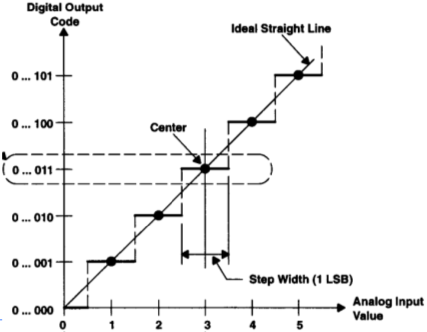
\includegraphics[scale=0.4]{ch3/image3.png}
	\captionof{figure}{ }
	\end{wrapfigure}
	\begin{equation}
	\left\{\begin{array}{ll}
	F_{xA} + F_{xB} &=0\\
	F_{yA} + F_{yB} &= 0\\
	LF_{yB} &=0
	\end{array}\right.
	\end{equation}\ \\
	
	
	\subsection{Équilibre des nœuds}
	\begin{wrapfigure}[7]{r}{6.5cm}
	\vspace{-4mm}
	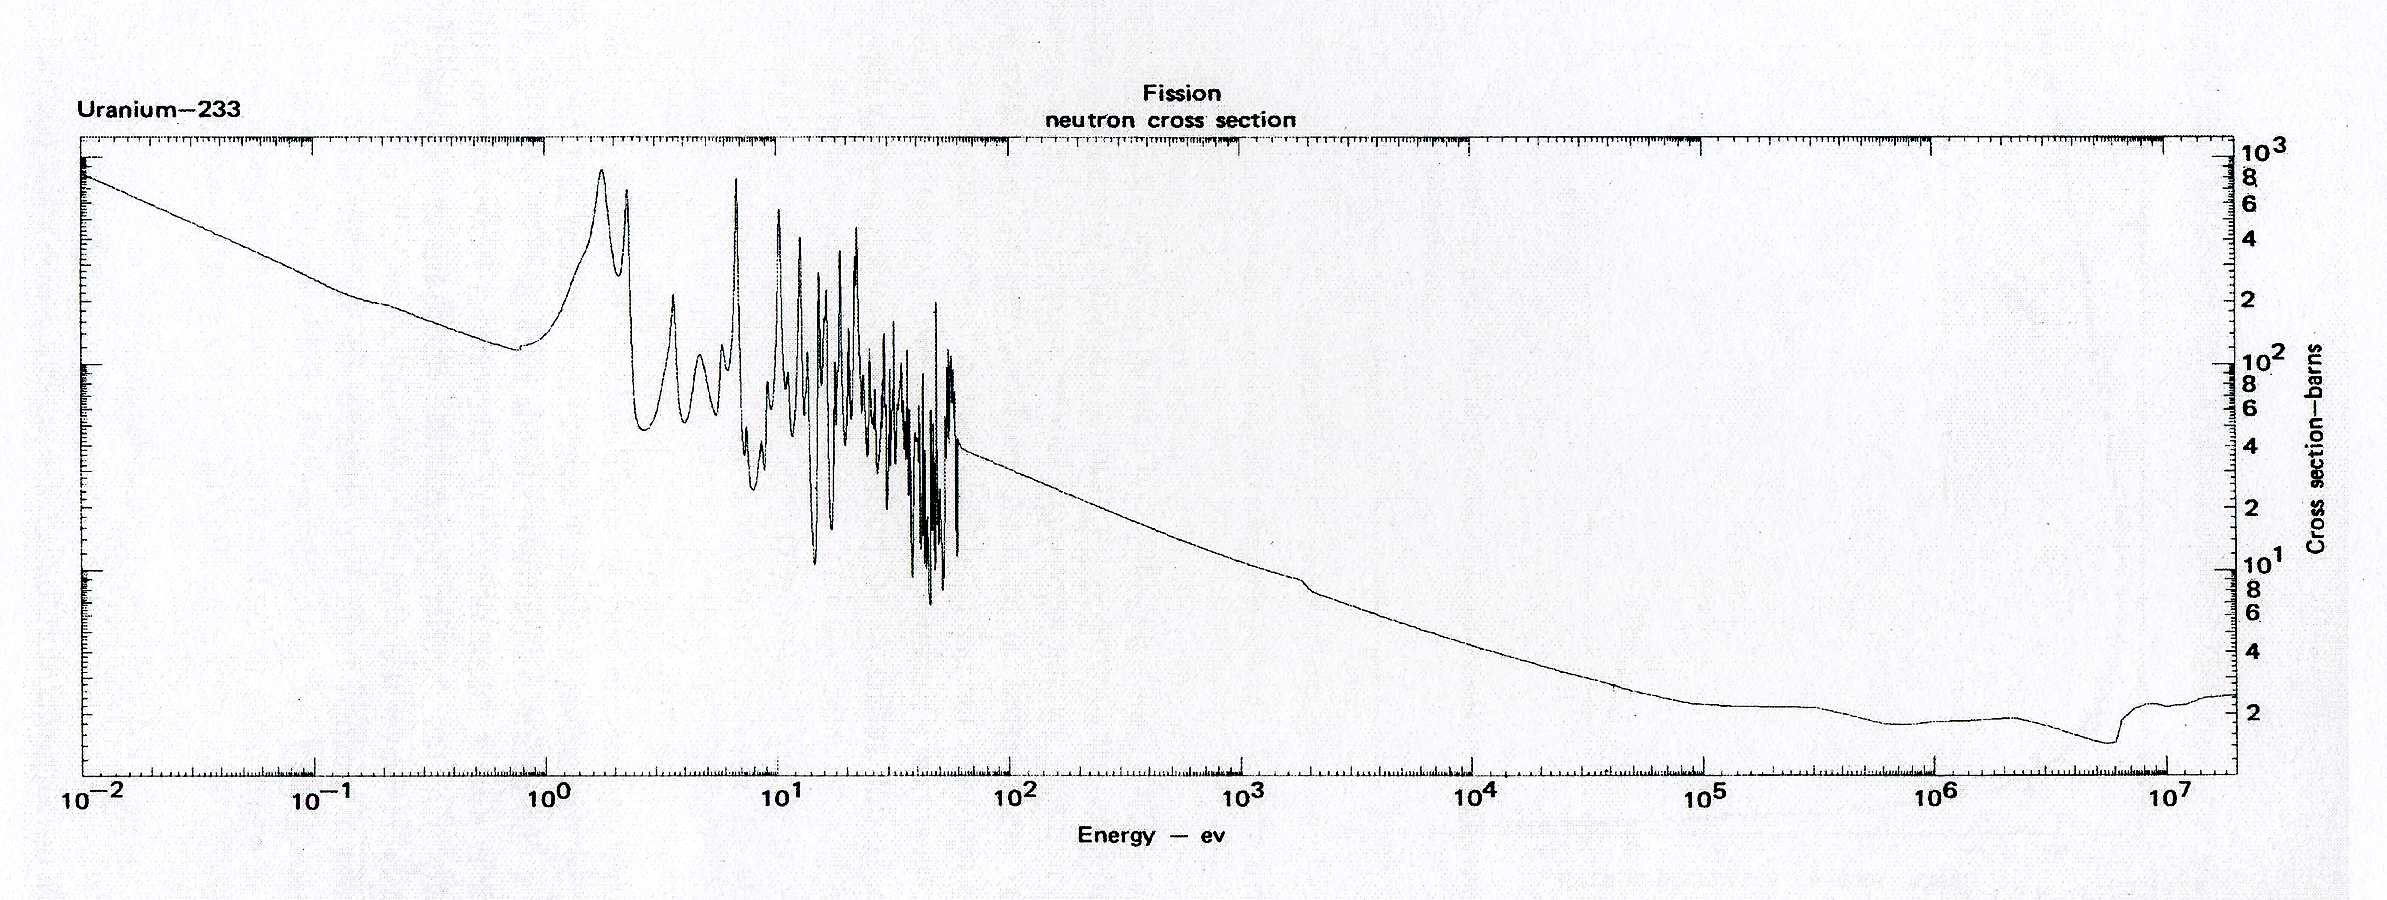
\includegraphics[scale=0.4]{ch3/image4.png}
	\captionof{figure}{ }
	\end{wrapfigure}
		Encore une fois rien de difficile, la méthode est systématique :
	\begin{itemize}
	\item[$\bullet$] Isoler un nœud en coupant les barres qui y aboutissent
	\item[$\bullet$] Appliquer les efforts normaux et les efforts extérieurs
	\item[$\bullet$] Écrire les équations d’équilibre du nœud
	\end{itemize}
	
	\subsection{Structure isostatique ?}
	La condition d'isostaticité est que le nombre d'inconnues statiques soit 
	égal au nombre d'équations d'équilibres. Nous avons :
	\begin{itemize}
	\item[$\bullet$] Nombre de barres : $b \rightarrow b$ efforts normaux 
	inconnus
	\item[$\bullet$] Nombre de RDL : $R \rightarrow R$ composantes de réactions 
	inconnues
	\item[$\bullet$] Nombre de nœuds : $n\rightarrow 2b$ équations d'équilibres 
	en 2D
	\end{itemize}
	Une structure est isostatique si (CN mais pas CNS) :
	\begin{equation}
	b + R = 2n
	\end{equation}
	\newpage
	
	\subsection{Coupe de Ritter}
		\subsubsection{Principe}
	\begin{wrapfigure}[7]{r}{7cm}
	\vspace{-4mm}
	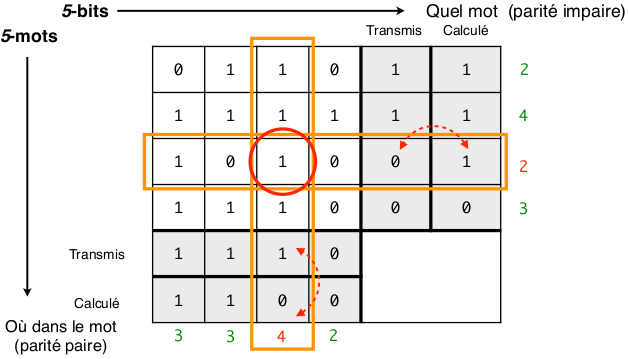
\includegraphics[scale=0.4]{ch3/image5.png}
	\captionof{figure}{ }
	\end{wrapfigure}
		On cherche à calculer l'effort normal dans une barre. On va
		\begin{itemize}
		\item[$\bullet$] Couper la structure en deux parties \textbf{disjointes}
		\item[$\bullet$] Écrire l'équilibre d'une des parties
		\item[$\bullet$] S'arranger que cet effort normal soit la seule inconnue
		\end{itemize}
		Les slides 24-25 montrent comment appliquer cette méthode.
		
	\subsection{Quelques nœuds particuliers}
	Certains nœuds particuliers permettent de gagner du temps dans les calculs.
	\begin{center}
	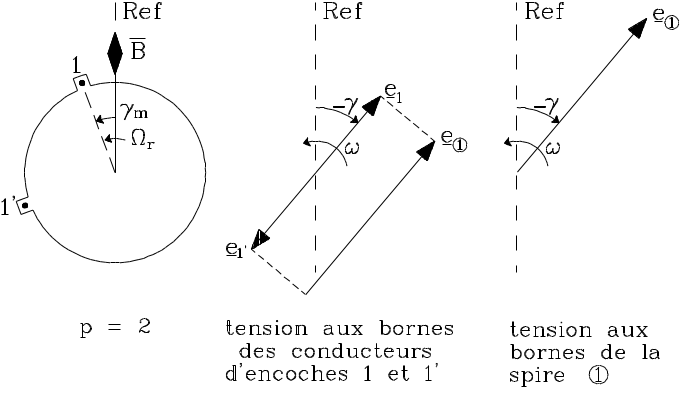
\includegraphics[scale=0.5]{ch3/image6.png}
	\captionof{table}{ }
	\end{center}
	
	
		\subsubsection{Barres à efforts nuls}
		\begin{wrapfigure}[9]{l}{7cm}
		\vspace{-6mm}
		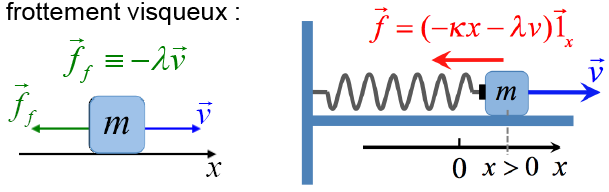
\includegraphics[scale=0.4]{ch3/image7.png}
		\captionof{figure}{ }
		\end{wrapfigure}
		En appliquant ce magnifique tableau et en l'appliquant sur la figure 
		ci-dessous, je peux déjà affirmer que pleins d'efforts normaux seront 
		nuls avant même de commencer à faire des calculs et donc gagner du 
		temps (qui, au vu de la longueur de l'examen peut être précieux).\\
		Notons que la barre du bas doit forcément être en traction, sans quoi 
		elle se "barrerait" (pfpfpf) avec le rouleau. 
		
	\subsection{Dilatation thermique}
	Il peut y avoir déformation axiale du à une élévation $\Delta T$ de la 
	température, déformation donnée par $\epsilon_{th} = \alpha\Delta T$. \\
	Si la structure est isostatique, elle est librement dilatable (car pas de 
	$T$ dans les équations d'équilibres) et son allongement est 
	\begin{equation}
	\Delta L_{th} = L\epsilon_{th} : L\alpha\Delta T
	\end{equation}
	Si la dilatation est empêchée, cela provoque un effort normal
	\begin{equation}
	N_{th} = -EA\epsilon_{th}\qquad\text{ou}\qquad N_{th} = -EA\alpha \Delta T
	\end{equation}

%%%%%%%%%%%%%%%%%
% Bibliographie %
%%%%%%%%%%%%%%%%%
%\newpage
%\chapter{Bibliographie}
%\nocite{*}
%\printbibliography[heading=none]

%%%%%%%%%%%
% Annexes %
%%%%%%%%%%%
\appendix
%\chapter{Annexe 1}
Coucou

\end{document}
